\section{Complicated Branching Structures}


In the preceding section, the research hypothesis has been tested by
the comparison of simple shapes. In the preceding section, the
research hypothesis has been tested by the comparison of simple
shapes. More complex branching structures, as shown in
Fig.~\ref{fig:G1_imgs} and Fig.~\ref{fig:G2_imgs}, are produced in
this section for further test and understanding of the survival
curve. The branching structures in the images are equal-area and
vertically symmetric, but the template in $G_1$ is shorter and
narrower than in $G_2$. In $G_i$, $i=1, 2$, the larger number of
iterations $j$, the more complicated structures $L_j$, $j=3, 4, 5, 6$,
with more nodes.




\subsection{Output Analysis of $S(n)$}

    
       \begin{figure}
        \centering
        
        \begin{subfigure}[b]{0.45\textwidth}
          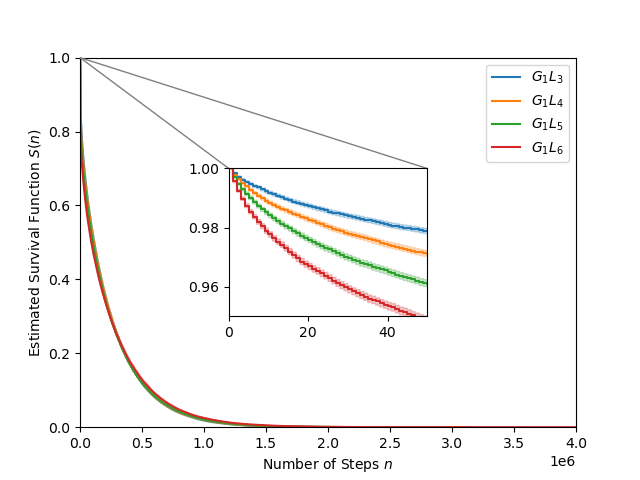
\includegraphics[width=\textwidth]{G_1_steps_sf.png}
          \caption{}
          \label{fig:sf_g1_branch_steps}
        \end{subfigure}
        \hfill
        \begin{subfigure}[b]{0.45\textwidth}
          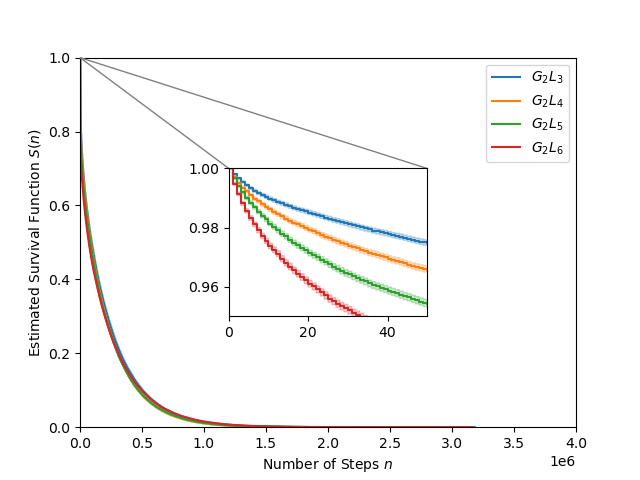
\includegraphics[width=\textwidth]{G_2_steps_sf.png}
          \caption{}
          \label{fig:sf_g2_branch_steps}
        \end{subfigure}

        \caption{(a) and (b) are survival functions for branching structures in $G_1$ and $G_2$, respectively. $n$ is the number of steps taken by the particle from the initial to the stop pixel in LRWs.}
        \label{fig:sf_branch_steps}

      \end{figure}

       
       The inset plot in Fig.~\ref{fig:sf_branch_steps} shows that the
       decay rates of $S(n)$ for $L_j$, $j=3, ..., 6$, are
       significantly distinct. The graphical representation of short
       time behaviours of survival functions is consistent with the
       analytical result since bigger $j$ results in the larger
       perimeter of the branching structure.


       \begin{figure}
         \centering
         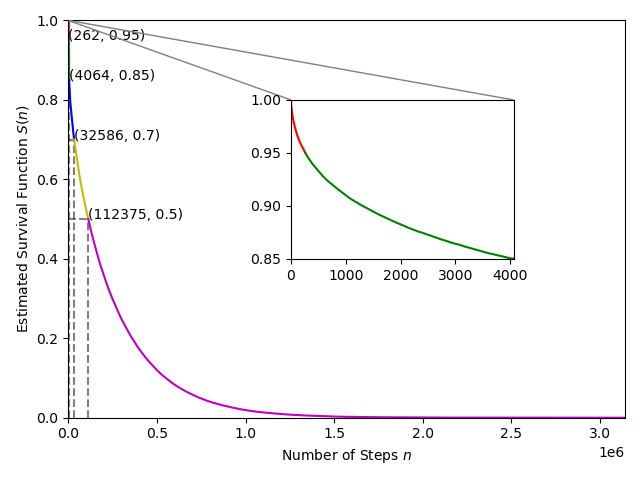
\includegraphics[width=\textwidth]{steps_seg_curve_G_1_L_3.png}
         \caption{It is the estimated survival function for LRWs in $G_1L_3$.}
         \label{fig:steps_seg_curve_G_1_L_3}
       \end{figure}

       
       As shown in Fig.~\ref{fig:steps_seg_curve_G_1_L_3}, the
       survival function is divided into several coloured segments. In
       Fig.~\ref{fig:G_1_L_3_steps_red_initial_pos_distribution},
       Fig.~\ref{fig:G_1_L_3_steps_green_initial_pos_distribution},
       Fig.~\ref{fig:G_1_L_3_steps_blue_initial_pos_distribution},
       Fig.~\ref{fig:G_1_L_3_steps_blue_initial_pos_distribution}, and
       Fig.~\ref{fig:G_1_L_3_steps_pink_initial_pos_distribution},
       particles' initial and stop positions are visualized by the
       scatter plots with the same colour as the segment to understand
       the underlying stochastic process and its properties. Moreover,
       the black region in the initial position plot is the target
       branching structure. 

       
       
       \begin{figure}
         \centering
         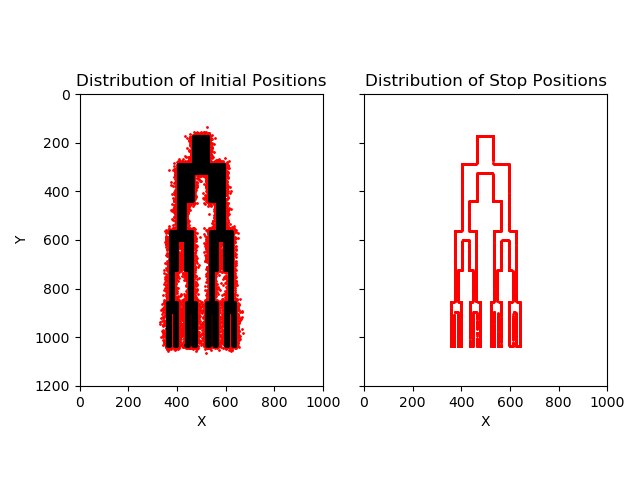
\includegraphics[width=\textwidth]{G_1_L_3_steps_red_initial_pos_distribution.png}
         \caption{$5\%$ of particles in the LRWs coloured by red will be absorbed within $262$ steps. The left subfigure tells us that their initial positions are distributed in the space closely surrounding the target branching structure. The right subfigure shows that the red particles describe the entire boundary of the object.}
         \label{fig:G_1_L_3_steps_red_initial_pos_distribution}
       \end{figure}



       \begin{figure}
         \centering
         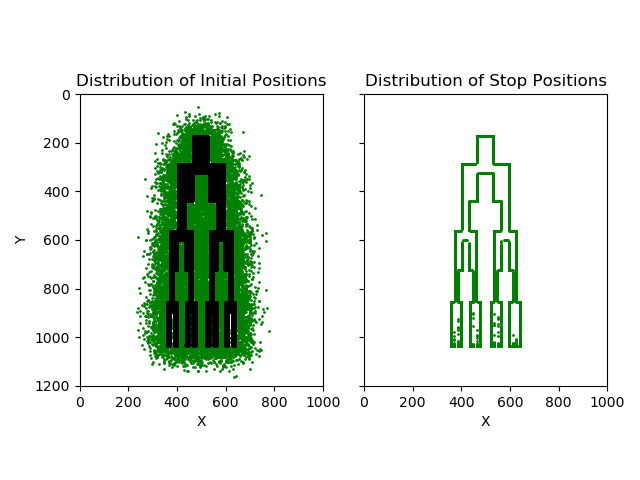
\includegraphics[width=\textwidth]{G_1_L_3_steps_green_initial_pos_distribution.png}
         \caption{Around $10$ percent of particles are near to the object, whose steps ranged from $262$ to $4064$. Compared with Fig.~\ref{fig:G_1_L_3_steps_red_initial_pos_distribution}, the green points also dispersed thoroughly between the branches. Nevertheless, some in-between area of the bottom limbs is empty. From the right plot, we can tell that particles can not characterize the whole boundary of the object since they can not encounter some parts of the edge of the bottom branches.}
         \label{fig:G_1_L_3_steps_green_initial_pos_distribution}
       \end{figure}


       \begin{figure}
         \centering
         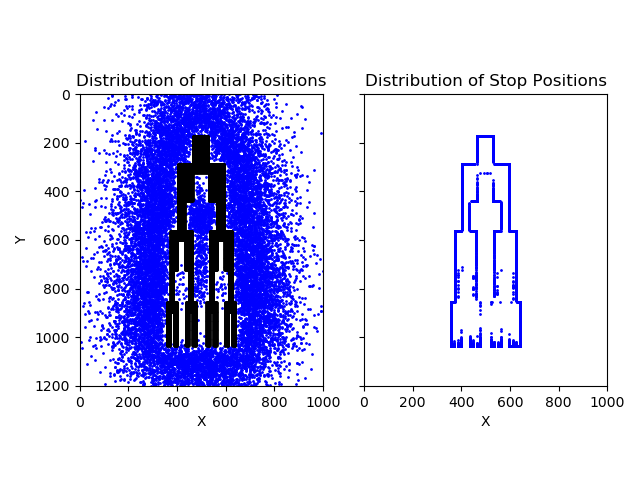
\includegraphics[width=\textwidth]{G_1_L_3_steps_blue_initial_pos_distribution.png}
         \caption{Approximate $15$ percent of particles originally started LRWs from the region a little bit far away from the target object. The number of steps for the blue particles is from 4064 to 32586. Not like the Fig.~\ref{fig:G_1_L_3_steps_green_initial_pos_distribution}, fewer particles are located in the area in-between the narrower branches. Moreover, if the initial sites of particles are further from the branching structure's external boundary, they will be more dispersive. Only some upper parts of the internal border can be depicted by the blue particles in the right subfigure. }
         \label{fig:G_1_L_3_steps_blue_initial_pos_distribution}
       \end{figure}
       

       \begin{figure}
         \centering
         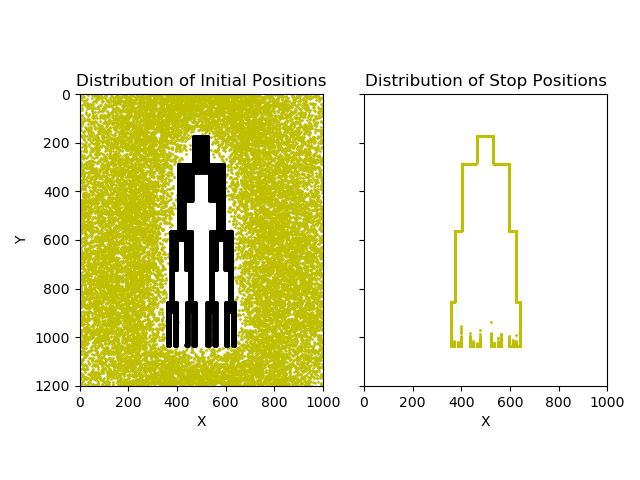
\includegraphics[width=\textwidth]{G_1_L_3_steps_y_initial_pos_distribution.png}
         \caption{The left subplot displays the initial positions of $60\%$ of particles in LRWs, which are distributed uniformly around the external outline of the branching structure. Moreover, none of them initially started walking from the space in-between the branches. Compared with the Fig.~\ref{fig:G_1_L_3_steps_blue_initial_pos_distribution}, the right subplot shows the object's entire external boundary and some internal border of its terminal limbs.}
         \label{fig:G_1_L_3_steps_yellow_initial_pos_distribution}
       \end{figure}


       \begin{figure}
         \centering
         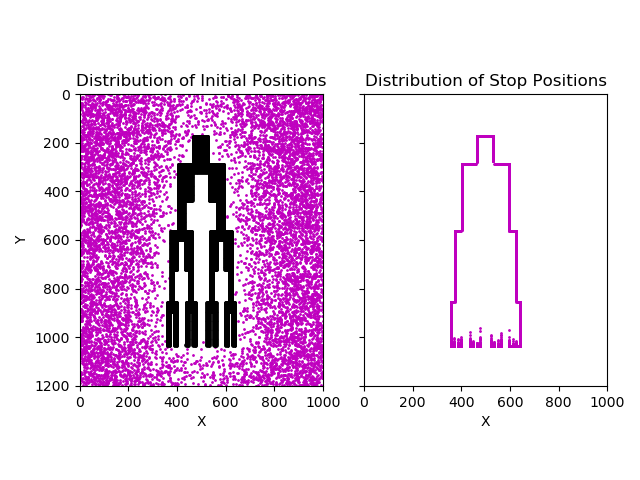
\includegraphics[width=\textwidth]{G_1_L_3_steps_m_initial_pos_distribution.png}
         \caption{Only $10$ percent of particles will still survive when their number of steps is bigger than $549701$. They are distributed initially from a region far away from the object and close to the image's edges. Similar to Fig.~\ref{fig:G_1_L_3_steps_yellow_initial_pos_distribution}, pink particles cannot delineate too much internal boundary of the branching structure.}
         \label{fig:G_1_L_3_steps_pink_initial_pos_distribution}
       \end{figure}


       In reality, LRWs is latent and cannot be observed
       directly. However, those scatter plots are the visual
       representations of revealing the first-passage properties of
       particles in LRWs. For example, particles will be absorbed in a
       shorter time if their initial positions are closer to the
       target because they have less randomness. Moreover, the broader
       and longer the in-between space of branches is, the more
       particles are generated with a larger variance for the number
       of steps. Therefore, each segment of the survival curve carries
       massive geometric and spatial information about the unoccupied
       area of the binary image (i.e. the region with black pixels)
       and the boundary of a simply connected domain (i.e. the
       artificial branching structure with white pixels).


       
      \begin{table}
        \centering
        \begin{tabular}{llrrrr}
          \toprule
                       &             &         &  p &    &     \\
          \cmidrule{3-6}
                       &             & Log-rank & TW & GB & FH  \\
          \midrule
          $G_1$ $L_3$  & $G_1$ $L_4$  &  0.4393 &  0.0285 &  0.0005 &  0.0005     \\
                       & $G_1$ $L_5$  & 0.0 & 0.0 & 0.0 & 0.0    \\
                       & $G_1$ $L_6$  & 0.0 & 0.0 & 0.0 & 0.0      \\
          $G_1$ $L_4$  & $G_1$ $L_5$  & 0.0007 & 0.0 & 0.0 & 0.0      \\
                       & $G_1$ $L_6$  & 0.0002 & 0.0 & 0.0 & 0.0       \\
          $G_1$ $L_5$   & $G_1$ $L_6$ & 0.7223 &  0.0 & 0.0 & 0.0      \\
          \bottomrule
        \end{tabular}
        \caption{The differences between the pairwise survival
          functions for branching objects in $G_1$ are statistically
          significant.}
         \label{tab:g1_ingroup_tests_steps}
      \end{table}


      \begin{table}
        \centering
        \begin{tabular}{llrrrr}
          \toprule
                       &             &         &  p &    &     \\
          \cmidrule{3-6}
                       &             & Log-rank & TW & GB & FH  \\
          \midrule
          $G_2$ $L_3$  & $G_2$ $L_4$  &  0.0 &  0.0 &  0.0 &  0.0     \\
                       & $G_2$ $L_5$  & 0.0 & 0.0 & 0.0 & 0.0    \\
                       & $G_2$ $L_6$  & 0.0 & 0.0 & 0.0 & 0.0      \\
          $G_2$ $L_4$  & $G_2$ $L_5$  & 0.0016 & 0.0 & 0.0 & 0.0      \\
                       & $G_2$ $L_6$  & 0.0004 & 0.0 & 0.0 & 0.0       \\
          $G_2$ $L_5$   & $G_2$ $L_6$ & 0.7199 &  0.0 & 0.0 & 0.0      \\
          \bottomrule
        \end{tabular}
        \caption{As mentioned before, the log-rank test will lose
          power if the proportional hazard assumption is
          violated. Except for the log-rank test, other statistical
          tests' results tell us that the pairwise survival functions
          are statistically different. }
        \label{tab:g2_ingroup_tests_steps}
      \end{table}
      

      Some weighted log-rank tests can be utilized to detect the early
      or late differences between the pairwise overlapping or crossing
      survival curves. In Table ~\ref{tab:g1_ingroup_tests_steps} and
      Table ~\ref{tab:g2_ingroup_tests_steps}, TW is the abbreviation
      for Tarone-Ware test, GB is for Gehan-Breslow test, and FH is
      for Fleming-Harrington test. However, p values in the tables are
      not too informative, and the log-rank test under conditions of
      non-proportional hazards leads to misleading results. Hence,
      distance measures are alternative methodologies for quantifying
      the discrepancy between survival functions.

      It is assumed that $\widehat S_1(t)$ and $\widehat S_2(t)$ are
      the Kaplan-Meier estimators of the survival functions for random
      variable $T_1 > 0$ and $T_2 > 0$, respectively. Let
      $(\tau_j)_{j=1, 2, ..., N}$ are distinct increasing observed
      times when the event of interest take place.

      In the vector space, the distance between $\widehat S_1(t)$ and
      $\widehat S_2(t)$ can be defined as the $L_p$ norm of their
      difference, $ 1 \leq p \leq \infty$, where

      \begin{equation}\label{eq:lp_norm}
        \begin{split}
          d_p(\widehat S_1(t), \widehat S_2(t))&= \lVert \widehat S_1(t) - \widehat S_2(t) \rVert_{p} \\
          &= \Big(\sum^{N}_{j=1} \lvert \widehat S_1(\tau_j) - \widehat S_2(\tau_j)\rvert^p\Big)^{\frac{1}{p}} \\
          &= \Big(\sum^{N}_{j=1} \lvert P({T_1 > \tau_j}) - P({T_2 > \tau_j}) \rvert^p\Big)^{\frac{1}{p}}
        \end{split}
      \end{equation}
      
      
      \begin{figure}
        \centering
        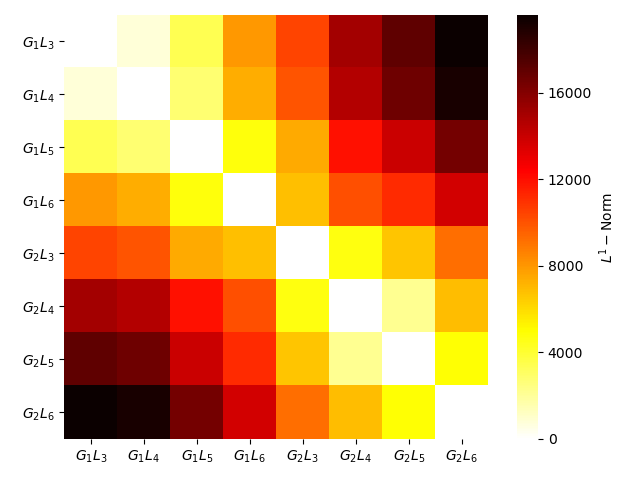
\includegraphics[width=\textwidth]{heatmap_ai_steps_l1.png}
        \caption{The distance matrix of pairwise survival functions
          for artificial images is visualized by a heat map, where
          $L^1$ norm is the distance metric.}
        \label{fig:heatmap_ai_steps_l1}
      \end{figure}


      As shown in Fig.~\ref{fig:heatmap_ai_steps_l1}, $p=1$ in
      Eq.~\ref{eq:lp_norm}, the dissimilarities between each pair of
      survival functions are measured by $d_1$ and depicted by colors
      in the heat map. The cells on the main diagonal are white
      because the distance of an object from itself is zero. The
      off-diagonal cells are symmetric, which are darker indicating
      more significant dissimilarities between survival functions or
      curves. In other words, the color of cells represents the
      variation in the shapes of branching structures in the
      artificial images.


      The top left and bottom right $4 \times 4$ cells are the
      in-group shape comparison of the branching structures. For each
      column, the cells become darker gradually since the objects in
      each group are more complicated as $j$ increase. The pale yellow
      cells adjacent to the diagonal, including $(G_1L3, G_1L4)$,
      $(G_1L4, G_1L5)$, $(G_1L5, G_1L6)$), $(G_2L3, G_2L4)$, $(G_2L4,
      G_2L5)$, and $(G_2L5, G_2L6)$), implies that the morphological
      changes are not dramatically different. Moreover, the top right
      and bottom left $4 \times 4$ cells are the between-group shape
      comparison. The smaller dissimilarities are closer to the
      diagonal, which gives a form of clustering the artificial
      images.

      
      In Fig.~\ref{fig:MDS_ai_steps_l1}, metric multidimensional
      scaling (MDS) \cite{borg2005modern} \cite{scikit-learn} is
      employed to display the distance matrix using a map defined in
      an abstract Cartesian space. It aims to represent objects as
      points in a low dimensional space so that distances between
      pairs of points match as well as possible the original
      dissimilarities calculated between the pairs of survival
      functions. For metric scaling, STRESS is a measure of the fit of
      the configuration of points representing the objects to the
      dissimilarities; a value of the STRESS of $20\%$ suggests a poor
      fit, $10\%$ fair, $5\%$ good and $2\%$ an excellent fit.

      \begin{figure}
        \centering
        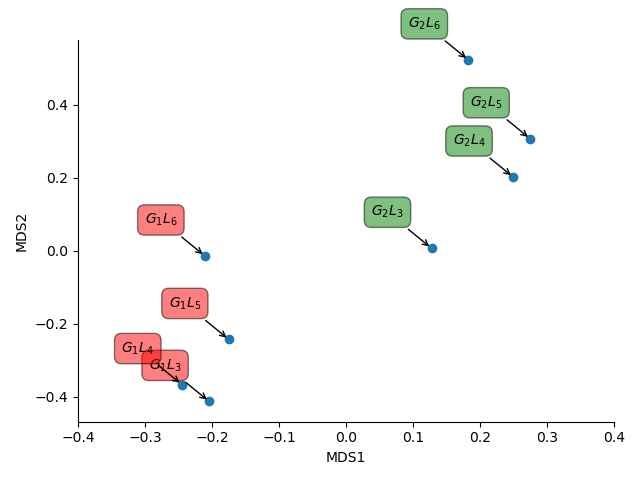
\includegraphics[width=\textwidth]{MDS_ai_steps_l1.png}
        \caption{The STRESS for the plot is about $8\%$. Points with
          green labels in the bottom left-hand corner represent the
          $G_1$ images, while others are $G_2$ images. It is easy to
          tell that there are two clusters for the artificial images,
          which coincide with reality.}
        \label{fig:MDS_ai_steps_l1}
      \end{figure}
      



       



       


























      

      %____________________________________________________________



       \newpage

       
      \subsubsection{$S(d)$}



      \begin{figure}
        \centering
        
        \begin{subfigure}[b]{0.45\textwidth}
          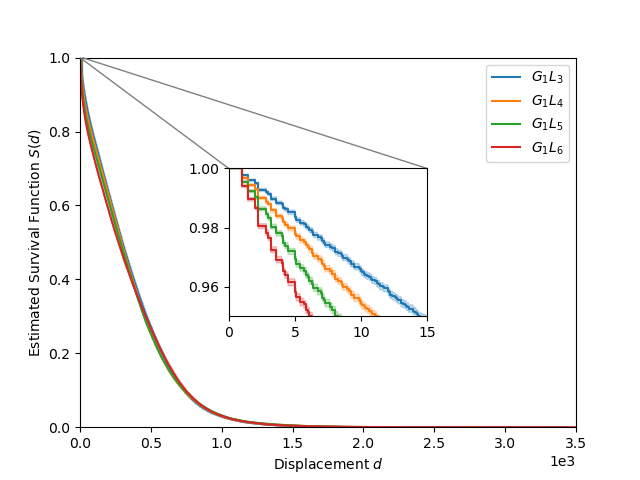
\includegraphics[width=\textwidth]{G_1_unwrap_disp_sf.png}
          \caption{}
          \label{fig:sf_g1_branch_disp}
        \end{subfigure}
        \hfill
        \begin{subfigure}[b]{0.45\textwidth}
          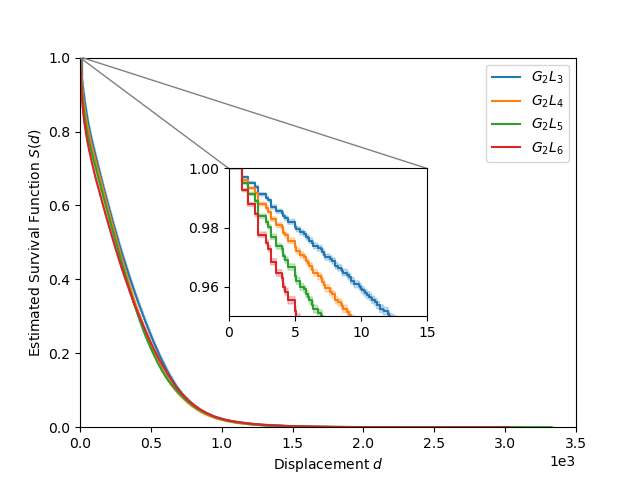
\includegraphics[width=\textwidth]{G_2_unwrap_disp_sf.png}
          \caption{}
          \label{fig:sf_g2_branch_disp}
        \end{subfigure}

        \caption{}
        \label{fig:sf_branch_disp}

      \end{figure}




      \begin{table}
        \centering
        \begin{tabular}{llrrrr}
          \toprule
                       &             &         &  p &    &     \\
          \cmidrule{3-6}
                       &             & Logrank & TW & GB & FH  \\
          \midrule
          $G_1$ $L_3$  & $G_1$ $L_4$  &  0.0 &  0.0 &  0.0 &  0.0     \\
                       & $G_1$ $L_5$  & 0.0 & 0.0 & 0.0 & 0.0    \\
                       & $G_1$ $L_6$  & 0.0 & 0.0 & 0.0 & 0.0      \\
          $G_1$ $L_4$  & $G_1$ $L_5$  & 0.0072 & 0.0 & 0.0 & 0.0      \\
                       & $G_1$ $L_6$  & 0.0003 & 0.0 & 0.0 & 0.0       \\
          $G_1$ $L_5$   & $G_1$ $L_6$ & 0.2883 &  0.0 & 0.0 & 0.0      \\
          \bottomrule
        \end{tabular}
        \label{tab:g1_ingroup_tests_disp}
        \caption{}
      \end{table}


      \begin{table}
        \centering
        \begin{tabular}{llrrrr}
          \toprule
                       &             &         &  p &    &     \\
          \cmidrule{3-6}
                       &             & Logrank & TW & GB & FH  \\
          \midrule
          $G_2$ $L_3$  & $G_2$ $L_4$  &  0.0 &  0.0 &  0.0 &  0.0     \\
                       & $G_2$ $L_5$  & 0.0 & 0.0 & 0.0 & 0.0    \\
                       & $G_2$ $L_6$  & 0.0 & 0.0 & 0.0 & 0.0      \\
          $G_2$ $L_4$  & $G_2$ $L_5$  & 0.0001 & 0.0 & 0.0 & 0.0      \\
                       & $G_2$ $L_6$  & 0.0015 & 0.0 & 0.0 & 0.0       \\
          $G_2$ $L_5$   & $G_2$ $L_6$ & 0.7019 &  0.0 & 0.0 & 0.0      \\
          \bottomrule
        \end{tabular}
        \label{tab:g2_ingroup_tests_disp}
        \caption{}
      \end{table}




      %______________________________________________________________
      

      \newpage
      

      \subsubsection{$S(R)$}
      
      \begin{figure}
        \centering
        
        \begin{subfigure}[b]{0.45\textwidth}
          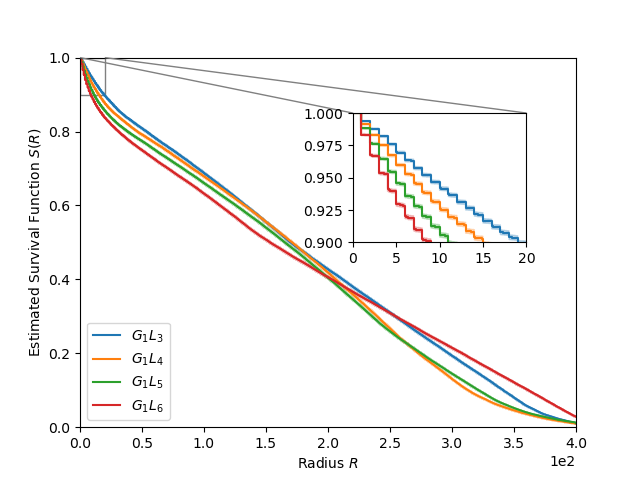
\includegraphics[width=\textwidth]{G_1_initial_radius_sf.png}
          \caption{}
          \label{fig:sf_g1_branch_radius}
        \end{subfigure}
        \hfill
        \begin{subfigure}[b]{0.45\textwidth}
          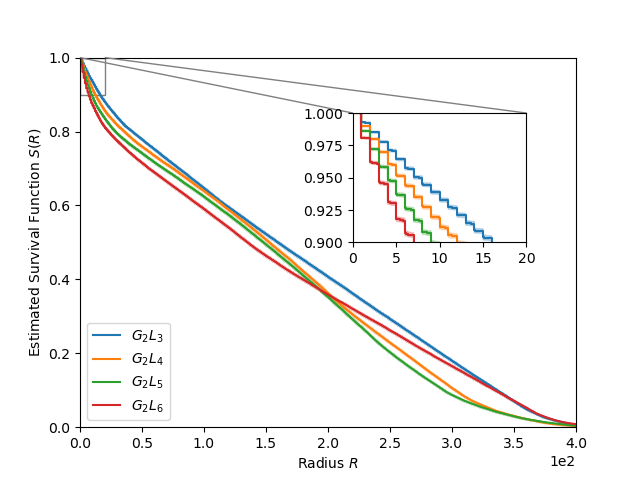
\includegraphics[width=\textwidth]{G_2_initial_radius_sf.png}
          \caption{}
          \label{fig:sf_g2_branch_radius}
        \end{subfigure}

        \caption{}
        \label{fig:sf_branch_radius}

      \end{figure}

      
      \begin{table}
        \centering
        \begin{tabular}{llrrrr}
          \toprule
                       &             &         &  p &    &     \\
          \cmidrule{3-6}
                       &             & Logrank & TW & GB & FH  \\
          \midrule
          $G_1$ $L_3$  & $G_1$ $L_4$  &  0.0 &  0.0 &  0.0 &  0.0     \\
                       & $G_1$ $L_5$  & 0.0 & 0.0 & 0.0 & 0.0    \\
                       & $G_1$ $L_6$  & 0.0 & 0.0 & 0.0 & 0.0      \\
          $G_1$ $L_4$  & $G_1$ $L_5$  & 0.1773 & 0.0 & 0.0 & 0.0      \\
                       & $G_1$ $L_6$  & 0.0 & 0.0 & 0.0 & 0.0       \\
          $G_1$ $L_5$   & $G_1$ $L_6$ & 0.0 &  0.0 & 0.0 & 0.0      \\
          \bottomrule
        \end{tabular}
        \label{tab:g1_ingroup_tests_radius}
        \caption{}
      \end{table}


      \begin{table}
        \centering
        \begin{tabular}{llrrrr}
          \toprule
                       &             &         &  p &    &     \\
          \cmidrule{3-6}
                       &             & Logrank & TW & GB & FH  \\
          \midrule
          $G_2$ $L_3$  & $G_2$ $L_4$  &  0.0 &  0.0 &  0.0 &  0.0     \\
                       & $G_2$ $L_5$  & 0.0 & 0.0 & 0.0 & 0.0    \\
                       & $G_2$ $L_6$  & 0.0 & 0.0 & 0.0 & 0.0      \\
          $G_2$ $L_4$  & $G_2$ $L_5$  & 0.0 & 0.0 & 0.0 & 0.0      \\
                       & $G_2$ $L_6$  & 0.0 & 0.0 & 0.0 & 0.0       \\
          $G_2$ $L_5$   & $G_2$ $L_6$ & 0.0 & 0.0 & 0.0253 & 0.0253      \\
          \bottomrule
        \end{tabular}
        \label{tab:g2_ingroup_tests_radius}
        \caption{}
      \end{table}


      


















    


      \newpage
      
    \subsection{Conclusion}

      \begin{itemize}
         \item In a short time, the survival function of rectangle decays faster than the circle, which conforms to the analytical results.
  
         \item The differences of estimated survival functions between circle and rectangle are statistically significant, which coincides with the real shape dissimilarities.

         \item Within a same group, when $t$ is small, the more branching the object is, the faster the survival function decays.

         \item Within a same group, the pairwise survival functions are statistically different.

         \item The corresponding target structures in $G_1$ and $G_3$ are invariant shapes under translation since their survival function are not statistically different. In other words, periodic boundary conditions of the image can eliminate the effect of the locations.

         \item LRWs can describe and classify the geometries, their spatial configurations, and the unoccupied area in the image.
    \end{itemize}




